\documentclass[../Main/main.tex]{subfiles}

\begin{document}
	\graphicspath{{../Time dependent equations/figs/}}
	\chapter{Time evolving equations}
	In this chapter we discuss numerical solving algorithms for parabolic equations with non-linearities, such as Richards' equation \eqref{eq:richards}. 

	
	\section*{Linearization}
	Now we have seen that the heat equation leads to a sequence of linear systems. In the same way, we expect that our non-linear Richards' equation \eqref{eq:richards} leads to a system of non-linear equations. We start by discussing this in a general setting
	\begin{equation}\label{eq:non-linear-problem}
		\text{find }x\in U \text{ such that }\pmb{f}(\pmb{x})=\pmb{0} \\ \text{ where } f:U\subset\mathbb{R}^n\rightarrow\mathbb{R}^n
	\end{equation}
	The solution in \eqref{eq:non-linear-problem} is called a \emph{root}, it is almost always found using an iterative method.\par 
	A common iterative scheme to solve \eqref{eq:non-linear-problem} is the \emph{Newton method}, let $D\pmb{f}(\pmb{x}_{j-1})^{-1}:\mathbb{R}^n\rightarrow\mathbb{R}^n$ be the Jacobian of $\pmb{f}(\pmb{x}_{j-1})$.
	\begin{equation}
		\pmb{x}_j = \pmb{x}_{j-1} -D\pmb{f}(\pmb{x}_{j-1})^{-1}\pmb{f}(\pmb{x}_{j-1})
	\end{equation}
	In one dimension a convergence proof i easily obtained by techniques from calculus, the following theorem is found in  slightly more detail in (Cheney\cite{Cheney}, chapter 3):
	\begin{theorem}
		Let $f''<2$ with $f(\overline{x})=0$ and $f'(x)> \delta \ \forall x \in B_{\epsilon}(\overline{x})$, then the Newton method is locally quadratic convergent:  For $x_0\in B_{\epsilon}(\overline{x})$ we have
		\begin{equation}
			| x_{j+1}-\overline{x}| \leq \frac{1}{\delta}|x_j - \overline{x}|^2< |x_j-\overline{x}|
		\end{equation}
	\end{theorem}
	\begin{proof}
		Define $e_n=x_n-\overline{x}$. Then we have by Taylor expansion
		\begin{equation}\label{eq:newton_taylor}
			0 = f(\overline{x})=f(x_j-e_j) = f(x_j)-f'(x_j)e_j + \frac{f''(\psi)e_j^2}{2}
		\end{equation}
		For some $\psi$ between $x_j$ and $\overline{x}$. Further we get by definition of the newton method
		\begin{equation}
			\begin{aligned}
				e_{j+1} = x_{j+1}-\overline{x} &= x_n-\frac{f(x_j)}{f'(x_j)}-\overline{x}\\
				&=e_j - \frac{f(x_j)}{f'(x_j)}\\ &= \frac{e_j f'(x_j)-f(x_j)}{f'(x_j)}
			\end{aligned}
		\end{equation}
		By the Taylor expansion around $x_j$, \eqref{eq:newton_taylor}, we get
		\begin{equation}
			e_{j+1} = \frac{e_j^2f''(\psi)}{2f'(x_j)}
		\end{equation}
	The assumptions on $f'$ and  $f''$ combined with $|e_0|<\delta$ give us the estimate
		\begin{equation}
			| e_{1} | \leq \frac{2}{2\delta}|e_0|^2<|e_0|
		\end{equation}
	By the same reasoning we get convergence
	\begin{equation}
		|e_{j+1}|<|e_j|
	\end{equation}
	And the quadratic convergence
	\begin{equation}
		| e_{j+1} | \leq \frac{1}{\delta}|e_j|^2
	\end{equation}
	\end{proof}
	For a similar result in more dimensions see (Knabner \cite{Knabner}, chapter 8). One apparent drawback of this method is that it's only locally convergent, ie. one needs to start the iteration in a neighbourhood of the root where the Jacobian is well defined. In practice one often solves the system
	\begin{equation}
		D\pmb{f}(\pmb{x}_{j-1})\pmb{\delta}_{j} = -\pmb{f}(\pmb{x}_{j-1})
	\end{equation}
	And then update the current iterate with $\pmb{x}_j = \pmb{x}_{j-1} + \pmb{\delta}_{j}$. One often end end up with a situation where the matrix $D\pmb{f}(\pmb{x}_{j-1})$ needs to be computed and assembled for every iteration. This may be computationally expensive. So Newtons method may be slow despite it's quadratic convergence, if it even converges.\par 
	A simpler approach is to swap the Jacobian with a diagonal matrix $L\pmb{I}$ such that 
	\begin{equation}\label{eq:L-scheme}
		L\pmb{\delta}_j = - \pmb{f}(\pmb{x}_{j-1})
	\end{equation}
	This is called the \emph{L-scheme}, and will be method we will use for linearization in this thesis. In one dimension it is easy to prove convergence:

	\begin{theorem}
		Let $f\in C(\mathbb{R})$ and $L>\sup_{x\in\mathbb{R}}f'(x)$, then the L-scheme converges linearly for all $x_0\in \mathbb{R}$.
	\end{theorem}
	\begin{proof}
		Define $e_j = e_j-\overline{x}$, then we get
		\begin{equation}
			e_{j+1} = x_j-\frac{f(x_j)}{L}-\overline{x}=e_j-\frac{f(x_j)}{L}
		\end{equation}
		We use the same trick as before with the Taylor expansion around the root.
		\begin{equation}
			0 = f(\overline{x}) = f(x_j-e_j) = f(e_j)-f'(\psi)e_j\Rightarrow e_j = \frac{f(x_j)}{f'(\psi)}
		\end{equation}
		Using this and the assumption on $L$ we get the estimate
		\begin{equation}
			|e_{j+1}|=|e_j(1-\frac{f'(\psi)f(x_j)}{f(x_j)L})|\leq|e_j||1-\frac{f'(\psi)}{L}|<|e_j|
		\end{equation}
	\end{proof}
	To see how this could be applied to parabolic PDE's we consider the equation:
	
	\section*{Richards' equation}
	\addcontentsline{toc}{section}{Richards' equation}
	We will first consider the non-linear, parabolic equation:
	\begin{equation}\label{eq:richards simple}
		\begin{aligned}[c]
			\partial_t \theta(u) - \nabla \cdot \kappa \nabla u &= q \\
			u &= g \\
			u &= u_0
		\end{aligned}
		\ \ \
		\begin{aligned}[c]
			x &\in \Omega  \\
			x &\in \partial \Omega \\
			x &\in \Omega  
		\end{aligned}
		\ \ \
		\begin{aligned}
			t&\in (0,T] \\
			t&\in (0,T] \\
			t&=0.
		\end{aligned}
	\end{equation}
	Which is similar to Richards' equation \eqref{eq:richards}, only without the gravity and non-linear permeability. We start by discretizing \eqref{eq:richards simple} with the MPFA-L method, we divide our domain into $d$ quadrilaterals. Writing \eqref{eq:semidiscrete FVM} in vector form we find $\tilde{u}_h \in \mathbb{R}^d$ such that:
	\begin{equation}
		\partial_t\pmb{B}^{V} \theta(\tilde{u}_h) + \pmb{A}^V \tilde{u}_h = \pmb{q}^V. 
	\end{equation}
	We can then discretize in time using backward euler. Given $ \tilde{u}_h^{n-1},\pmb{q}^n \in \mathbb{R}^d$ we should then find $ \tilde{u}_h^n \in \mathbb{R}^d$ such that: 
	\begin{equation} \label{eq:non-linear richards FVM}
		\pmb{B}^V  \theta(\tilde{u}_h)^n + \tau \pmb{A}^V \tilde{u}_h^n = \tau \pmb{q}^{Vn} + \pmb{B}^V  \theta(\tilde{u}_h)^{n-1}.
	\end{equation}
	Now we need to linearize \eqref{eq:non-linear richards FVM} with the L-scheme. We see from \eqref{eq:L-scheme} that the applying this linearization leads to the equation:
	\begin{equation}\label{eq:linearized richards fvm}
		L\pmb{B}^V(\tilde{u}^{n,j}_h-\tilde{u}^{n,j-1}_h) + \tau \pmb{A} \tilde{u}_h^{n,j} = -\pmb{B}^V \theta (\tilde{u}_h^{n,j-1})  + \tau \pmb{q}^{Vn} +  \pmb{B}^V \theta (\tilde{u}_h^{n-1}).
	\end{equation}
	The above equation can be solved for $\tilde{u}_h^{n,j}$, and is in principal the same as solving \eqref{eq:stationary_heat} which we have proved equivalence with the modified finite element method for.
	Now let us see how it would look if we discretized \eqref{eq:richards simple} with the modified finite element method. Let $u_h, v_h\in V_h$, where $V_h$ is defined as piecewise linear functions as in definition \ref{def:linear ansatz}. Then our semidisrectization would be to find $u_h \in V_h$ such that
	\begin{equation}
		\left \langle \partial_t\hat{I}_h \theta(u_h^n),\hat{I}_h v_h \right \rangle_0 + \left \langle \kappa \nabla u^n_h, \nabla v_h \right \rangle_0 = \left \langle q,v_h \right \rangle_0 \ \ \forall v_h \in V_h.
	\end{equation}
	Next we would discretize in time, our discretization now reads; given $u_h^{n-1} \in V_h$ find $u_h \in V_h$
	\begin{equation}
		\left \langle \hat{I}_h \theta(u_h^n),\hat{I}_h v_h \right \rangle_0 +\tau \left \langle \kappa \nabla u^n_h, \nabla v_h \right \rangle_0 = \tau \left \langle q^n,\hat{I}_h v_h \right \rangle_0 + \left \langle \hat{I}_h u_h^{n-1},\hat{I}_h v_h \right \rangle_0
	\end{equation}
	for all $v_h \in V_h$. Finally we also linearize this with the L-scheme. Following the same procedure as for \eqref{eq:linearized richards fvm} we get; given  $u_h^{n-1},u_h^{n,j-1} \in V_h$ find $u_h^{n,j} \in V_h$ such that
	\begin{equation}\label{eq:linearized richards fem}
		\begin{aligned}
			&L \left \langle \hat{I}_h u^{n,j}_h -  \hat{I}_h u^{n,j-1}_h,\hat{I}_h v_h \right \rangle_0 + \tau \left \langle \kappa \nabla u^{n,j}_h,\nabla v_h \right \rangle \\&=\tau \left \langle q^n,\hat{I}_h v_h \right \rangle_0 + \left \langle \hat{I}_h u_h^{n-1},\hat{I}_h v_h \right \rangle_0 -\left \langle \hat{I}_h \theta(u^{n,j-1}_h),\hat{I}_h v_h \right \rangle_0
		\end{aligned}
	\end{equation}
	for all $v_h \in V_h$. Since the mass matrix is diagonal with our modified finite element method, we can express \eqref{eq:linearized richards fem} as a matrix-vector equation similar to the MPFA-L method \eqref{eq:linearized richards fvm}. Let $\hat{u}_h^{n,j} \in \mathbb{R}^d$ be the coefficients that together with the basis functions make up $u_h^{n,j} \in V_h$. Then our \eqref{eq:richards simple} discretized with modified finite elements in space, backward euler in time and L-scheme linearization reads; given $\hat{u}_h^{n,j-1},\hat{u}_h^{n-1} \in \mathbb{R}^d$ find  $\hat{u}_h^{n,j} \in \mathbb{R}^d$ such that 
	\begin{equation}\label{eq:linearized richards fem system}
		L\pmb{B}(\hat{u}^{n,j}_h-\hat{u}^{n,j-1}_h) + \tau \pmb{A} \hat{u}_h^{n,j} = -\pmb{B} \theta (\hat{u}_h^{n,j-1})  + \tau \pmb{q}^n +  \pmb{B} \theta (\hat{u}_h^{n-1}).
	\end{equation}
	We can now state an important result for obtaining a convergence estimate for Richards' equation.
	\begin{lemma}
		The system \eqref{eq:linearized richards fvm} obtain from MPFA-L method for discretizing the simplified Richards' equation \eqref{eq:richards simple}, is equivalent to the one obtained with the modified finite element method \eqref{eq:linearized richards fem system}. Moreover we have the equalities: 
		\begin{equation}
			\pmb{A}^V = \pmb{A}, \ \ \ \pmb{B}^V = \pmb{B}, \ \ \ \pmb{q}^V = \pmb{q}, \ \ \ \hat{u}_h = \tilde{u}_h
		\end{equation}
		\begin{proof}
			\todo[inline]{todo}
			follows from equivalence chapter.
		\end{proof}
	\end{lemma}
	How this fit in with the convergence proof for Richards' equation with MPFA can be seen in the figure below.
	\begin{figure}[H]
		\centering
		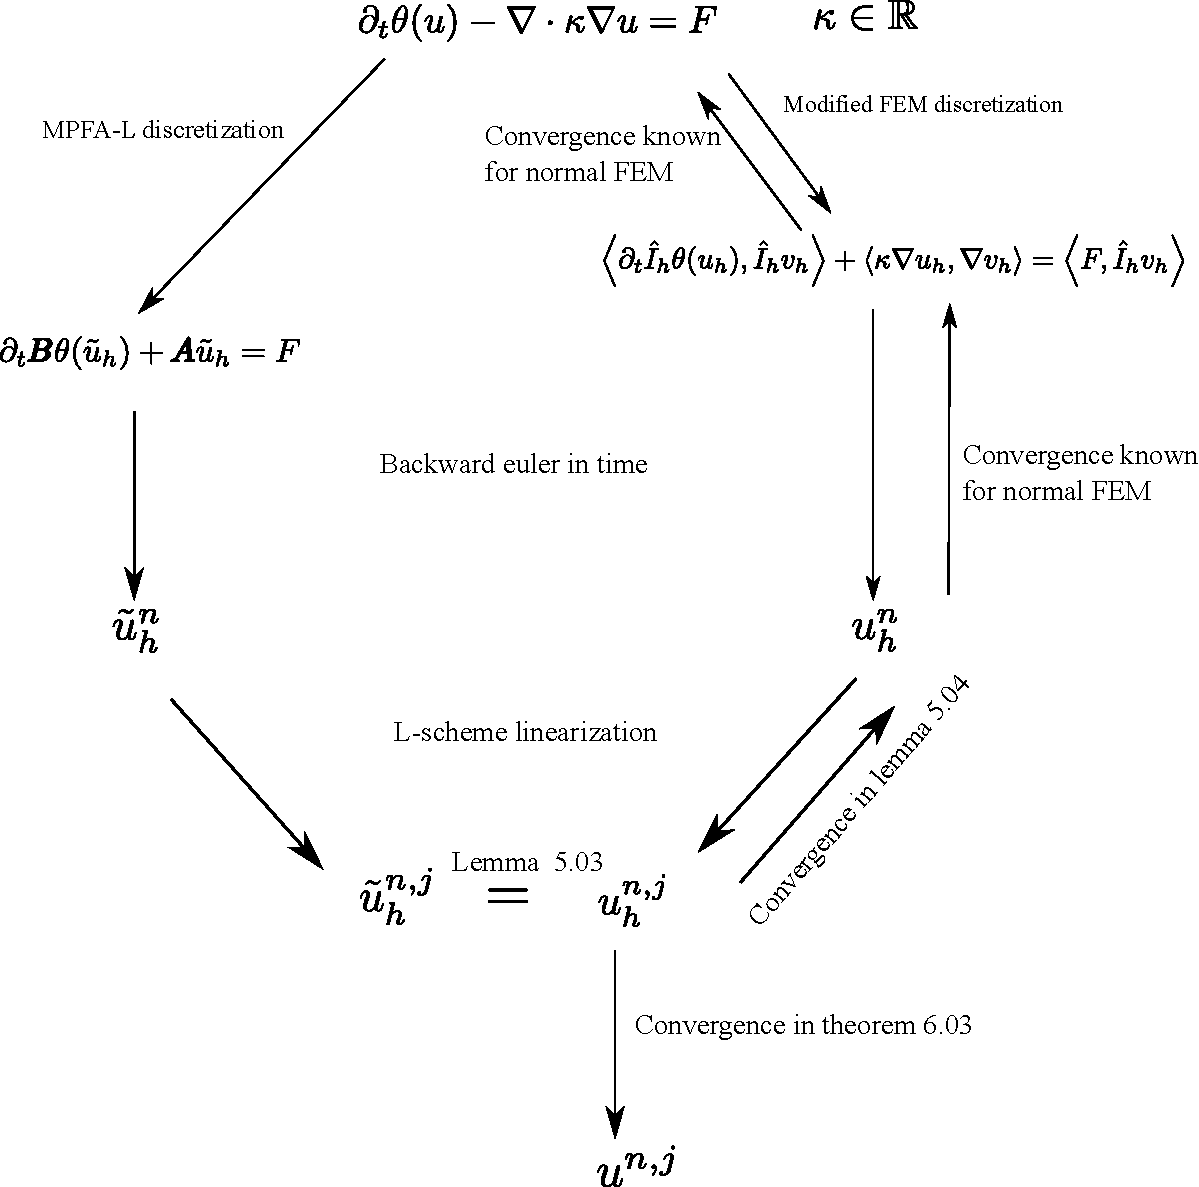
\includegraphics[width=0.8\textwidth]{homogenous_sumary.pdf}
	\end{figure}
	
	We still need to prove that \eqref{eq:linearized richards fem} converges to a fixed point as $j\rightarrow \infty$. This is done (List, Radu, 2016,\cite{list2016study}) for the normal finite element method, but we do the proof here for our modified finite element method. 
	First we need assumptions on the parametrizations $\kappa $ and $\theta$:
	\begin{itemize}
		\item[\textbf{A 1}] The water content parametrization $\theta(\cdot)$ is monotonically increasing with $sup|\theta'| = L_{\theta}$ and Lipschitz continuos.
		\item[\textbf{A 2}] The permeability $\kappa$ is positive. 
	\end{itemize}
	\begin{theorem}
		Assume \textbf{A 1} and \textbf{A 2} above and that the constant L is chosen such that $L \geq L_{\theta}$. Then the L-scheme \eqref{eq:L-scheme-FEM} converges linearly. 
	\end{theorem}
	\begin{proof}
		Let as before $e^{n,j} = u^{n,j}-u^n$ be the iteration error.
		We start by subtracting \eqref{eq:richards_timedisc} from \eqref{eq:L-scheme-FEM} and obtain:
			\begin{equation}
			\begin{aligned}
				\left \langle \hat{I}_h \theta(u^{n,j-1}_h) - \hat{I}_h \theta(u^{n}_h),\hat{I}_h v_h \right \rangle_0 &+ L \left \langle \hat{I}_h e^{n,j}_h -  \hat{I}_h e^{n,j-1}_h,\hat{I}_h v_h \right \rangle_0 \\+ \tau \left \langle \kappa (\nabla u^{n,j}_h-\nabla u^{n}_h),\nabla v_h \right \rangle_0 &=0 
			\end{aligned}
		\end{equation}
		Now we test with $v_h=e^{n,j}$:
		\begin{equation}
			\begin{aligned}
				\left \langle \hat{I}_h \theta(u^{n,j-1}_h) - \hat{I}_h \theta(u^{n}_h),\hat{I}_h e^{n,j} \right \rangle_0 &+ L \left \langle \hat{I}_h e^{n,j}_h -  \hat{I}_h e^{n,j-1}_h,\hat{I}_h e^{n,j} \right \rangle_0 \\+ \tau \left \langle \kappa\nabla e^{n,j},\nabla e^{n,j} \right \rangle_0 &=0 
			\end{aligned}
		\end{equation}
		We use the identity $\left \langle x-y,x\right \rangle = \frac{1}{2}\left \| x \right \|^2 + \frac{1}{2}\left \| x-y \right \|^2 - \frac{1}{2} \left \| y \right \|^2$ and some algebraic manipulation to obtain:
		\begin{equation}
			\begin{gathered}
					\left \langle \hat{I}_h \theta(u^{n,j-1}_h) - \hat{I}_h \theta(u^{n}_h),\hat{I}_h e^{n,j-1} \right \rangle + 	\left \langle \hat{I}_h \theta(u^{n,j-1}_h) - \hat{I}_h \theta(u^{n}_h),\hat{I}_h e^{n,j} - \hat{I}_h e^{n,j-1}\right \rangle \\
					+\frac{L}{2}\left \| \hat{I} e^{n,j}\right \|^2 + \frac{L}{2}\left \| \hat{I} e^{n,j}-\hat{I}e^{n,j-1} \right \|^2 -\frac{L}{2}\left \| \hat{I} e^{n,j-1}\right \|^2 \\
				+ \tau \left \langle \kappa \nabla e^{n,j},\nabla e^{n,j} \right \rangle_0 =0 
			\end{gathered}
		\end{equation}
		Then we put some terms on the right hand side:
		\begin{equation}
			\begin{gathered}
				\left \langle \hat{I}_h \theta(u^{n,j-1}_h) - \hat{I}_h \theta(u^{n}_h),\hat{I}_h e^{n,j-1} \right \rangle +\frac{L}{2}\left \| \hat{I} e^{n,j}\right \|^2 	 \\
				 + \frac{L}{2}\left \| \hat{I} e^{n,j}-\hat{I}e^{n,j-1} \right \|^2 + 
				\tau \left \langle \kappa\nabla e^{n,j},\nabla e^{n,j} \right \rangle_0  = \\ - \left \langle \hat{I}_h \theta(u^{n,j-1}_h) - \hat{I}_h \theta(u^{n}_h),\hat{I}_h e^{n,j} - \hat{I}_h e^{n,j-1}\right \rangle+\frac{L}{2}\left \| \hat{I} e^{n,j-1}\right \|^2
			\end{gathered}
		\end{equation}
		Now we use the Cauchy Swarchz inequality, and the monotonicity $\textbf{A 1}$ on the first term. Similarly we use Cauchy Swarchz and $\textbf{A 2}$ on the second term. Finally we use Young's inequality on the first term on the right hand side.
		\begin{equation}
			\begin{gathered}
				\frac{1}{L_{\theta}}\left \| \hat{I}_h (\theta(u^{n,j-1}-\theta(u^{n}))) \right \|^2 + \frac{L}{2}\left \| \hat{I} e^{n,j}\right \|^2 \\
				+ \frac{L}{2}\left \| \hat{I} e^{n,j}-\hat{I}e^{n,j-1} \right \|^2 + \tau \kappa_m \left \| \nabla e^{n,j} \right \|^2 \\
				\leq \frac{1}{2L} \left \| \hat{I}_h(\theta (u^{n,j-1})-\theta (u^n) ) \right \|^2  + \frac{L}{2} \left \|\hat{I}_h( e^{n,j} - e^{n,j-1}) \right \|^2+\frac{L}{2}\left \| \hat{I} e^{n,j-1}\right \|^2
			\end{gathered}
		\end{equation} 
		Next we can use Poincare inequality:
		\begin{equation}\label{eq:L-proof}
			\begin{gathered}
				\frac{L}{2}\left \| \hat{I}_h e^{n,j}\right\|^2 + \frac{\tau \kappa_m}{C_{\Omega}} \left \|e^{n,j} \right \|^2 \leq (\frac{1}{2L} - \frac{1}{L_{\theta}}) \left \| \hat{I}_h(\theta (u^{n,j-1}-\theta (u^n))) \right \|^2 +\frac{L}{2}\left \| \hat{I} e^{n,j-1}\right \|^2
			\end{gathered}
		\end{equation}
		Since $L_{\theta} \leq L$ we can remove the first term on the right side from the inequality. We can also use the lemma \ref{lemma:int_error} about the interpolation error:
		\begin{equation}
			\left \| \hat{I}_h e^{n,j} \right \|^2 = \left \| \hat{I}_h e^{n,j} - e^{n,j} + e^{n,j} \right \|^2 \leq (ch\left \| e^{n,j}\right \| + \left \| e^{n,j} \right \|)^2=(1+ch)^2\left \| e^{n,j} \right \|^2
		\end{equation}
		Now \eqref{eq:L-proof} becomes:
		\begin{equation}
			(\frac{L}{2}+\frac{\tau \kappa_m }{C_{\Omega}(1 + ch)^2})\left \| \hat{I}_h e^{n,j} \right \|^2 \leq \frac{L}{2} \left \| \hat{I}_h e^{n,j-1}\right \|^2
		\end{equation}
	\end{proof}
	
\end{document}